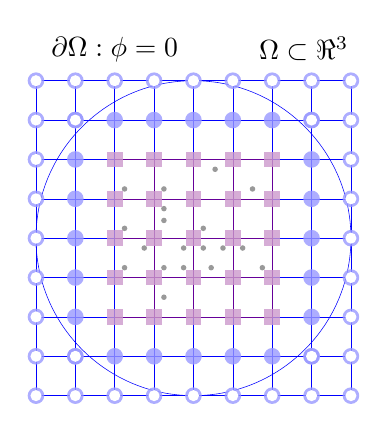
\begin{tikzpicture}[domain=-0.2:4.2,scale=1.0]
    \draw[very thin,color=blue,step=5mm] (0.0,0.0) grid (4,4);
    \draw[very thin,color=red,step=5mm,opacity=0.4] (1.0,0.99) grid (3,3);
    %\draw[very thin,color=gray,step=2.5mm] (0.5,-0.2) grid (3.5,1.5);
    
    %\filldraw[fill=gray!20,fill opacity=0.8](2,2)--(2,3)--(3,3)--(3,2)--cycle;

    %curved boundart
    %\draw (-0.2,3.55) to[out=20,in=180] node [sloped,below] {} (4.2,3.8);
    %\draw (-0.2,3.3) to[out=30,in=180] node [sloped,below] {$\Omega$} (4.2,3.8);
    
    %\coordinate [label=above:\C] (C) at (intersection of B and 1,0--1,1);
    %\fill[black,opacity=.5] C circle (2pt);
    
    \draw[very thin,color=blue] (2.0,2.0) circle (2);
  
    %labels
    \node at (3.4,4.4) {$\Omega \subset \Re^3$};
    \node at (1,4.4) {$\partial \Omega: \phi = 0$};

    \foreach \i in {0, 0.5, ..., 4}
    {
        \fill[blue!40,opacity=0.8] (\i,0.0) circle (3pt);
        \fill[white,opacity=1.0] (\i,0.0) circle (2pt);
    }
    \foreach \i in {0.5, 1.0, ..., 3.5}
    {
        \fill[blue!40,opacity=0.8] (\i,0.5) circle (3pt);
    }

    \foreach \i in {0.5, 1.0, ..., 3.5}
    {
        \fill[blue!40,opacity=0.8] (\i,3.5) circle (3pt);
    }
    \foreach \i in {0, 0.5, ..., 4}
    {
        \fill[blue!40,opacity=0.8] (\i,4.0) circle (3pt);
        \fill[white,opacity=1.0] (\i,4.0) circle (2pt);
    }
    
    \foreach \i in {1, 1.5, ..., 3}
    {
        \fill[blue!40,opacity=0.8] (0.0,\i) circle (3pt);
        \fill[white,opacity=1.0] (0.0,\i) circle (2pt);
    }
    \foreach \i in {1, 1.5, ..., 3}
    {
        \fill[blue!40,opacity=0.8] (0.5,\i) circle (3pt);
    }
    \foreach \i in {1, 1.5, ..., 3}
    {
        \fill[blue!40,opacity=0.8] (3.5,\i) circle (3pt);
    }
    \foreach \i in {1, 1.5, ..., 3}
    {
        \fill[blue!40,opacity=0.8] (4.0,\i) circle (3pt);
        \fill[white,opacity=1.0] (4.0,\i) circle (2pt);
    }
    \fill[blue!40,opacity=0.8] (3.5,3.5) circle (3pt);
    \fill[white,opacity=1.0] (3.5,3.5) circle (2pt);
    \fill[blue!40,opacity=0.8] (4.0,3.5) circle (3pt);
    \fill[white,opacity=1.0] (4.0,3.5) circle (2pt);
    
    \fill[blue!40,opacity=0.8] (0.5,3.5) circle (3pt);
    \fill[white,opacity=1.0] (0.5,3.5) circle (2pt);
    \fill[blue!40,opacity=0.8] (0.0,3.5) circle (3pt);
    \fill[white,opacity=1.0] (0.0,3.5) circle (2pt);
    
    \fill[blue!40,opacity=0.8] (3.5,0.5) circle (3pt);
    \fill[white,opacity=1.0] (3.5,0.5) circle (2pt);
    \fill[blue!40,opacity=0.8] (4.0,0.5) circle (3pt);
    \fill[white,opacity=1.0] (4.0,0.5) circle (2pt);
    
    \fill[blue!40,opacity=0.8] (0.5,0.5) circle (3pt);
    \fill[white,opacity=1.0] (0.5,0.5) circle (2pt);
    \fill[blue!40,opacity=0.8] (0.0,0.5) circle (3pt);
    \fill[white,opacity=1.0] (0.0,0.5) circle (2pt);
        
   
    \foreach \j in {1, 1.5, ..., 3}
    {
        \foreach \i in {1, 1.5, ..., 3}
        {
            \fill[violet!40,opacity=0.8] (\i-0.1,\j-0.1) rectangle (\i+0.1,\j+0.1);
        }
    }

    %\fill[violet!40,opacity=0.8] (-0.1,0.9) rectangle (0.1,1.1);
    %\fill[violet!40,opacity=0.8] (0.4,0.9) rectangle (0.6,1.1);
    %\fill[violet!40,opacity=0.8] (0.9,0.9) rectangle (1.1,1.1);

    %particles
    \fill[black!40] (2.225,1.625) circle (1pt);
    \fill[black!40] (2.750,2.625) circle (1pt);
    \fill[black!40] (1.625,1.25) circle (1pt);
    
    \fill[black!40] (2.275,2.875) circle (1pt);

    \fill[black!40] (1.625,2.625) circle (1pt);
    
    \fill[black!40] (1.375,1.875) circle (1pt);

    \fill[black!40] (1.125,2.625) circle (1pt);
    \fill[black!40] (1.125,2.125) circle (1pt);
    \fill[black!40] (1.125,1.625) circle (1pt);
    
    \fill[black!40] (1.625,2.375) circle (1pt);
    \fill[black!40] (1.625,1.625) circle (1pt);
    \fill[black!40] (1.625,2.225) circle (1pt);

    \fill[black!40] (1.875,1.875) circle (1pt);
    \fill[black!40] (1.875,1.625) circle (1pt);
    
    \fill[black!40] (2.125,1.875) circle (1pt);
    \fill[black!40] (2.125,2.125) circle (1pt);

    \fill[black!40] (2.375,1.875) circle (1pt);

    \fill[black!40] (2.625,1.875) circle (1pt);
    
    \fill[black!40] (2.875,1.625) circle (1pt);

\end{tikzpicture}
